\documentclass{standalone}
\usepackage{tikz}
\usetikzlibrary{patterns, positioning}
\usepackage[sfdefault]{ClearSans} %% option 'sfdefault' activates Clear Sans as the default text font
\usepackage[T1]{fontenc}

\begin{document}
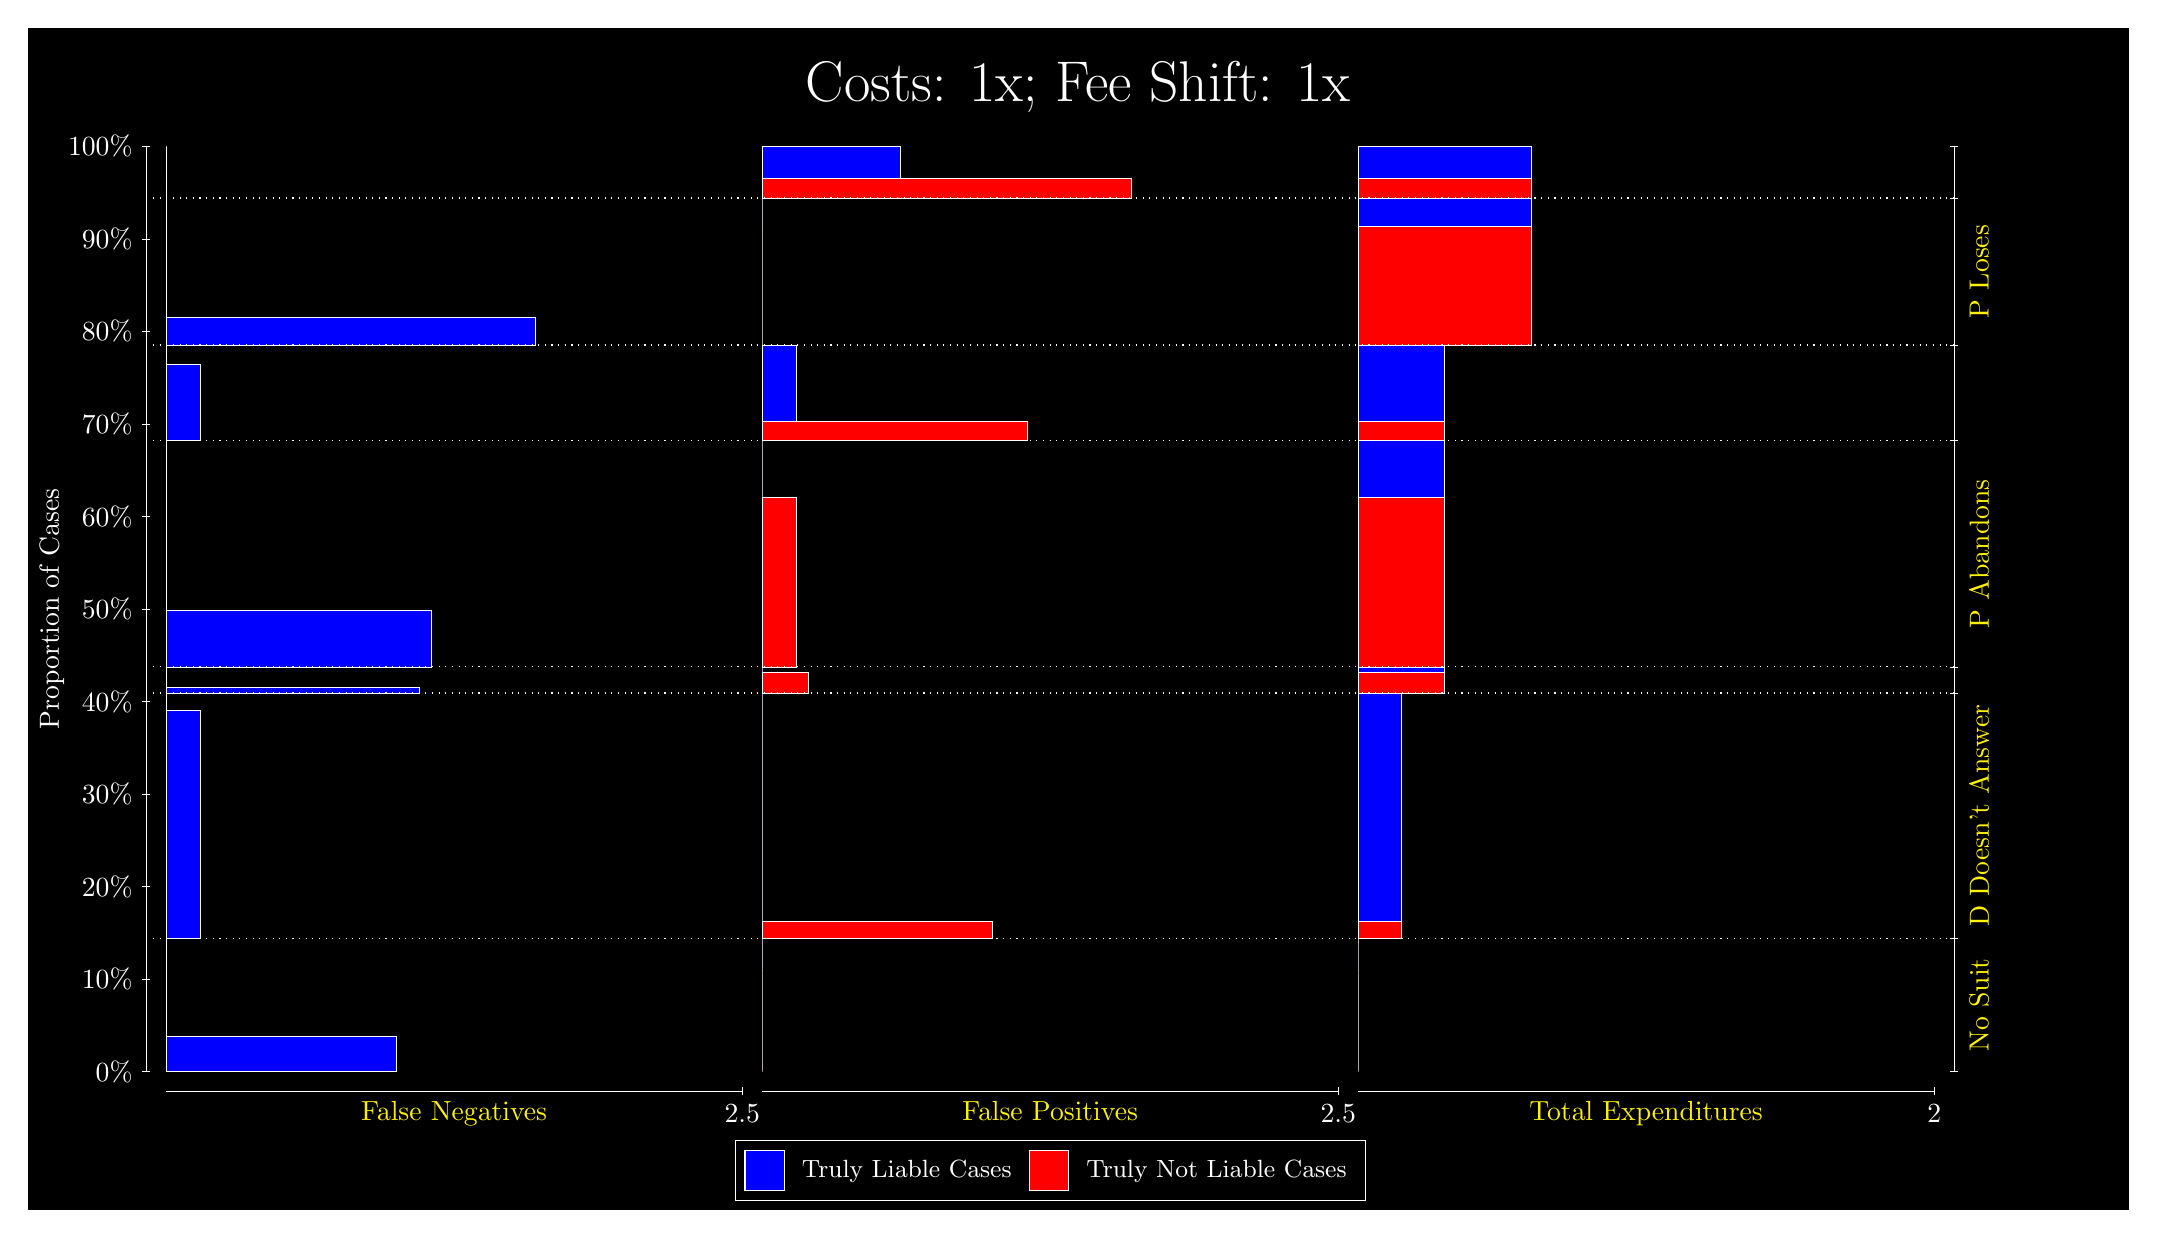
\begin{tikzpicture}
\draw[fill=black] (0,0) rectangle (26.667,15);
\draw[text=white] (0,13.5) rectangle (26.667,15) node[midway] {\huge Costs: 1x; Fee Shift: 1x};
\draw[white, very thin] (1.5,1.75) -- (1.5,13.5);
\node[rotate=90, text=white, anchor=center] at (0.3, 7.625) {Proportion of Cases};
\draw[white, very thin] (1.45,1.75) -- (1.55,1.75);
\node[text=white, anchor=east] at (1.45, 1.75) {0\%};
\draw[white, very thin] (1.45,2.925) -- (1.55,2.925);
\node[text=white, anchor=east] at (1.45, 2.925) {10\%};
\draw[white, very thin] (1.45,4.1) -- (1.55,4.1);
\node[text=white, anchor=east] at (1.45, 4.1) {20\%};
\draw[white, very thin] (1.45,5.275) -- (1.55,5.275);
\node[text=white, anchor=east] at (1.45, 5.275) {30\%};
\draw[white, very thin] (1.45,6.45) -- (1.55,6.45);
\node[text=white, anchor=east] at (1.45, 6.45) {40\%};
\draw[white, very thin] (1.45,7.625) -- (1.55,7.625);
\node[text=white, anchor=east] at (1.45, 7.625) {50\%};
\draw[white, very thin] (1.45,8.8) -- (1.55,8.8);
\node[text=white, anchor=east] at (1.45, 8.8) {60\%};
\draw[white, very thin] (1.45,9.975) -- (1.55,9.975);
\node[text=white, anchor=east] at (1.45, 9.975) {70\%};
\draw[white, very thin] (1.45,11.15) -- (1.55,11.15);
\node[text=white, anchor=east] at (1.45, 11.15) {80\%};
\draw[white, very thin] (1.45,12.325) -- (1.55,12.325);
\node[text=white, anchor=east] at (1.45, 12.325) {90\%};
\draw[white, very thin] (1.45,13.5) -- (1.55,13.5);
\node[text=white, anchor=east] at (1.45, 13.5) {100\%};

\draw[white, very thin] (24.457,1.75) -- (24.457,13.5);
\draw[white, very thin] (24.407,1.75) -- (24.507,1.75);
\node[anchor=west] at (24.407, 1.75) {};
\draw[white, very thin] (24.407,3.4404) -- (24.507,3.4404);
\node[anchor=west] at (24.407, 3.4404) {};
\draw[white, very thin] (24.407,6.5568) -- (24.507,6.5568);
\node[anchor=west] at (24.407, 6.5568) {};
\draw[white, very thin] (24.407,6.8894) -- (24.507,6.8894);
\node[anchor=west] at (24.407, 6.8894) {};
\draw[white, very thin] (24.407,9.7623) -- (24.507,9.7623);
\node[anchor=west] at (24.407, 9.7623) {};
\draw[white, very thin] (24.407,10.977) -- (24.507,10.977);
\node[anchor=west] at (24.407, 10.977) {};
\draw[white, very thin] (24.407,12.844) -- (24.507,12.844);
\node[anchor=west] at (24.407, 12.844) {};
\draw[white, very thin] (24.407,13.5) -- (24.507,13.5);
\node[anchor=west] at (24.407, 13.5) {};

\draw[white, very thin, fill=blue] (1.75,1.75) rectangle (4.6775,2.1982);
\draw[white, very thin, fill=red] (1.75,2.1982) rectangle (1.75,3.4404);
\draw[white, very thin, fill=blue] (1.75,3.4404) rectangle (2.1891,6.3359);
\draw[white, very thin, fill=red] (1.75,6.3359) rectangle (1.75,6.5568);
\draw[white, very thin, fill=blue] (1.75,6.5568) rectangle (4.9703,6.6297);
\draw[white, very thin, fill=red] (1.75,6.6297) rectangle (1.75,6.8894);
\draw[white, very thin, fill=blue] (1.75,6.8894) rectangle (5.1167,7.6131);
\draw[white, very thin, fill=red] (1.75,7.6131) rectangle (1.75,9.7623);
\draw[white, very thin, fill=blue] (1.75,9.7623) rectangle (2.1891,10.735);
\draw[white, very thin, fill=red] (1.75,10.735) rectangle (1.75,10.977);
\draw[white, very thin, fill=blue] (1.75,10.977) rectangle (6.4341,11.335);
\draw[white, very thin, fill=red] (1.75,11.335) rectangle (1.75,12.844);
\draw[white, very thin, fill=red] (1.75,12.844) rectangle (1.75,13.096);
\draw[white, very thin, fill=blue] (1.75,13.096) rectangle (1.75,13.5);
\draw[white, very thin, fill=red] (9.3189,1.75) rectangle (9.3189,2.9923);
\draw[white, very thin, fill=blue] (9.3189,2.9923) rectangle (9.3189,3.4404);
\draw[white, very thin, fill=red] (9.3189,3.4404) rectangle (12.246,3.6613);
\draw[white, very thin, fill=blue] (9.3189,3.6613) rectangle (9.3189,6.5568);
\draw[white, very thin, fill=red] (9.3189,6.5568) rectangle (9.9044,6.8165);
\draw[white, very thin, fill=blue] (9.3189,6.8165) rectangle (9.3189,6.8894);
\draw[white, very thin, fill=red] (9.3189,6.8894) rectangle (9.758,9.0387);
\draw[white, very thin, fill=blue] (9.3189,9.0387) rectangle (9.3189,9.7623);
\draw[white, very thin, fill=red] (9.3189,9.7623) rectangle (12.686,10.004);
\draw[white, very thin, fill=blue] (9.3189,10.004) rectangle (9.758,10.977);
\draw[white, very thin, fill=red] (9.3189,10.977) rectangle (9.3189,12.486);
\draw[white, very thin, fill=blue] (9.3189,12.486) rectangle (9.3189,12.844);
\draw[white, very thin, fill=red] (9.3189,12.844) rectangle (14.003,13.096);
\draw[white, very thin, fill=blue] (9.3189,13.096) rectangle (11.075,13.5);
\draw[white, very thin, fill=red] (16.888,1.75) rectangle (16.888,2.9923);
\draw[white, very thin, fill=blue] (16.888,2.9923) rectangle (16.888,3.4404);
\draw[white, very thin, fill=red] (16.888,3.4404) rectangle (17.437,3.6613);
\draw[white, very thin, fill=blue] (16.888,3.6613) rectangle (17.437,6.5568);
\draw[white, very thin, fill=red] (16.888,6.5568) rectangle (17.986,6.8165);
\draw[white, very thin, fill=blue] (16.888,6.8165) rectangle (17.986,6.8894);
\draw[white, very thin, fill=red] (16.888,6.8894) rectangle (17.986,9.0387);
\draw[white, very thin, fill=blue] (16.888,9.0387) rectangle (17.986,9.7623);
\draw[white, very thin, fill=red] (16.888,9.7623) rectangle (17.986,10.004);
\draw[white, very thin, fill=blue] (16.888,10.004) rectangle (17.986,10.977);
\draw[white, very thin, fill=red] (16.888,10.977) rectangle (19.083,12.486);
\draw[white, very thin, fill=blue] (16.888,12.486) rectangle (19.083,12.844);
\draw[white, very thin, fill=red] (16.888,12.844) rectangle (19.083,13.096);
\draw[white, very thin, fill=blue] (16.888,13.096) rectangle (19.083,13.5);
\draw[white, dotted] (1.5,3.4404) -- (24.457,3.4404);
\draw[white, dotted] (1.5,6.5568) -- (24.457,6.5568);
\draw[white, dotted] (1.5,6.8894) -- (24.457,6.8894);
\draw[white, dotted] (1.5,9.7623) -- (24.457,9.7623);
\draw[white, dotted] (1.5,10.977) -- (24.457,10.977);
\draw[white, dotted] (1.5,12.844) -- (24.457,12.844);
\draw[white, very thin] (1.75,1.5) -- (9.0689,1.5);
\node[text=yellow, anchor=north] at (5.4094, 1.5) {False Negatives};
\draw[white, very thin] (9.0689,1.45) -- (9.0689,1.55);
\node[text=white, anchor=north] at (9.0689, 1.45) {2.5};

\draw[white, very thin] (9.3189,1.5) -- (16.638,1.5);
\node[text=yellow, anchor=north] at (12.978, 1.5) {False Positives};
\draw[white, very thin] (16.638,1.45) -- (16.638,1.55);
\node[text=white, anchor=north] at (16.638, 1.45) {2.5};

\draw[white, very thin] (16.888,1.5) -- (24.207,1.5);
\node[text=yellow, anchor=north] at (20.547, 1.5) {Total Expenditures};
\draw[white, very thin] (24.207,1.45) -- (24.207,1.55);
\node[text=white, anchor=north] at (24.207, 1.45) {2};

\node[text=yellow, centered, rotate=90] at (24.777, 2.5952) {No Suit};
\node[text=yellow, centered, rotate=90] at (24.777, 4.9986) {D Doesn't Answer};

\node[text=yellow, centered, rotate=90] at (24.777, 8.3259) {P Abandons};

\node[text=yellow, centered, rotate=90] at (24.777, 11.911) {P Loses};


\draw (12.978300999999998,1.5) node[draw=none] (baseCoordinate) {};
\begin{scope}[align=center]
        \matrix[scale=0.5, draw=white, below=0.5cm of baseCoordinate, nodes={draw}, column sep=0.1cm]{
            \node[rectangle, draw, minimum width=0.5cm, minimum height=0.5cm, fill=blue] {}; &
            \node[draw=none, font=\small, text=white] (B) {Truly Liable Cases}; &
            \node[rectangle, draw, minimum width=0.5cm, minimum height=0.5cm, fill=red] {}; &
            \node[draw=none, font=\small, text=white] (B) {Truly Not Liable Cases}; \\
            };
\end{scope}

\end{tikzpicture}
\end{document}